\chapter{Graphical Models}
Mathematics, statistics, physics, and other academic fields have useful notational systems. As a hybrid of these and other disciplines, machine learning borrows from many of the existing systems. Notational abstractions are important to enable consistent and efficient communication of ideas, for both teaching and knowledge creation purposes. Much of machine learning revolves around modeling data processes, and then performing inference over those models to generate useful insights. In this chapter, we will be introducing a notational system known as the directed graphical model (DGM) that will help us reason about a broad class of models.

\section{Motivation}
Up until this point, we've defined notation on the fly, relied on common statistical concepts, and used diagrams to convey meaning about the problem setup for different techniques. We've built up enough working knowledge and intuition at this point to switch to a more general abstraction for defining models: directed graphical models (DGMS). DGMs will allow us to both consolidate our notation and convey information about arbitrary problem formulations. An example of what a DGM looks like for a linear regression problem setup is given in Figure \ref{fig:lin-reg-dgm}, and over the course of the chapter, we'll explain how to interpret the symbols in this diagram.
\begin{figure}
    \centering
    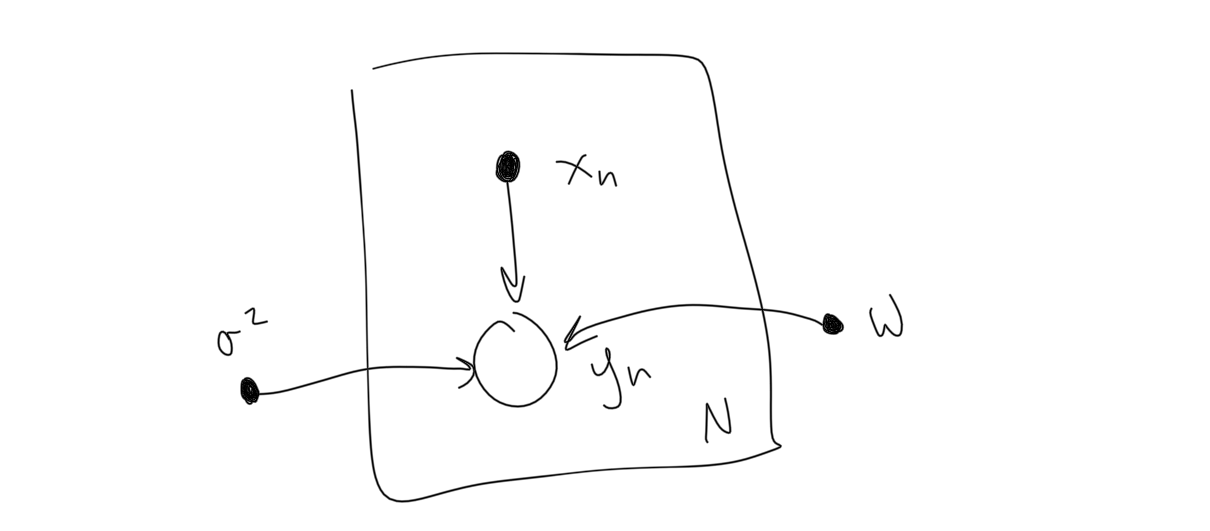
\includegraphics[width=0.5\paperwidth]{../GraphicalModels/fig/LinearRegressionDGM.png}
    \caption{Linear regression model expressed with a DGM.}
    \label{fig:lin-reg-dgm}
\end{figure}

We need graphical models for a couple of reasons. First, and most importantly, a graphical model unambiguously conveys a problem setup. This is useful both to share models between people (communication) and to keep all the information in a specific model clear in your own head (consolidation). Once we understand the meaning of the symbols in a DGM, it will be far easier to examine one of them than it will be to read several sentences describing the type of model we're imagining for a specific problem. Another reason we use DGMs is that they help us reason about independence properties between different parts of our model. For simple problem setups this may be easy to keep track of in our heads, but as we introduce more complicated models it will be useful to reason about independence properties simply by examining the DGM describing that model.

Ultimately, directed graphical models are a tool to boost efficiency and clarity. We'll examine the core components of a DGM, as well as some of their properties regarding independence and model complexity. The machinery we develop here will be used heavily in the coming chapters.

\section{Directed Graphical Models (Bayesian Networks)}
There are a few fundamental components to all of the models we've examined so far. In fact, we can model just about everything we've discussed to this point using just random variables, deterministic parameters, and arrows to indicate the relationships between them. Let's consider linear regression as a simple but comprehensive example. We have a random variable $y_n$, the object of predictive interest, which depend on deterministic parameters in the form of data $\textbf{x}_n$ and weights $\textbf{w}$. This results in the DGM given by Figure \ref{fig:lin-reg-dgm}. There are four primary pieces of notation that the linear regression setup gives rise to, and these four components form the backbone of every DGM we would like to construct.

\begin{figure}
    \centering
    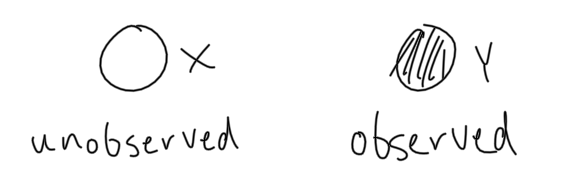
\includegraphics[width=0.5\paperwidth]{../GraphicalModels/fig/RandomVar.png}
    \caption{Random variables are denoted with an open circle, and it is shaded if the variable is observed.}
    \label{fig:random-var}
\end{figure}
\begin{figure}
    \centering
    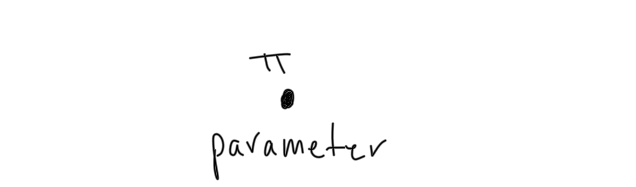
\includegraphics[width=0.5\paperwidth]{../GraphicalModels/fig/DeterministicParam.png}
    \caption{Deterministic parameters are denoted with a tight, small dot.}
    \label{fig:deterministic-param}
\end{figure}
\begin{figure}
    \centering
    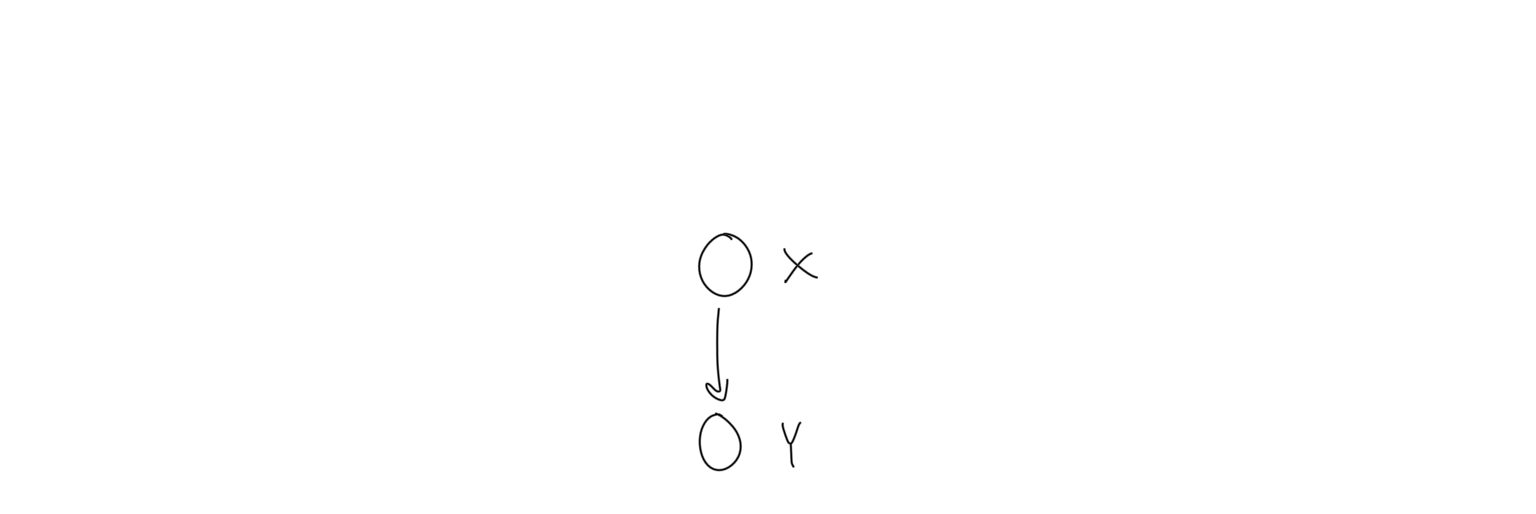
\includegraphics[width=0.7\paperwidth]{../GraphicalModels/fig/arrows.png}
    \caption{Arrows indicate dependence relationships.}
    \label{fig:arrows}
\end{figure}
\begin{figure}
    \centering
    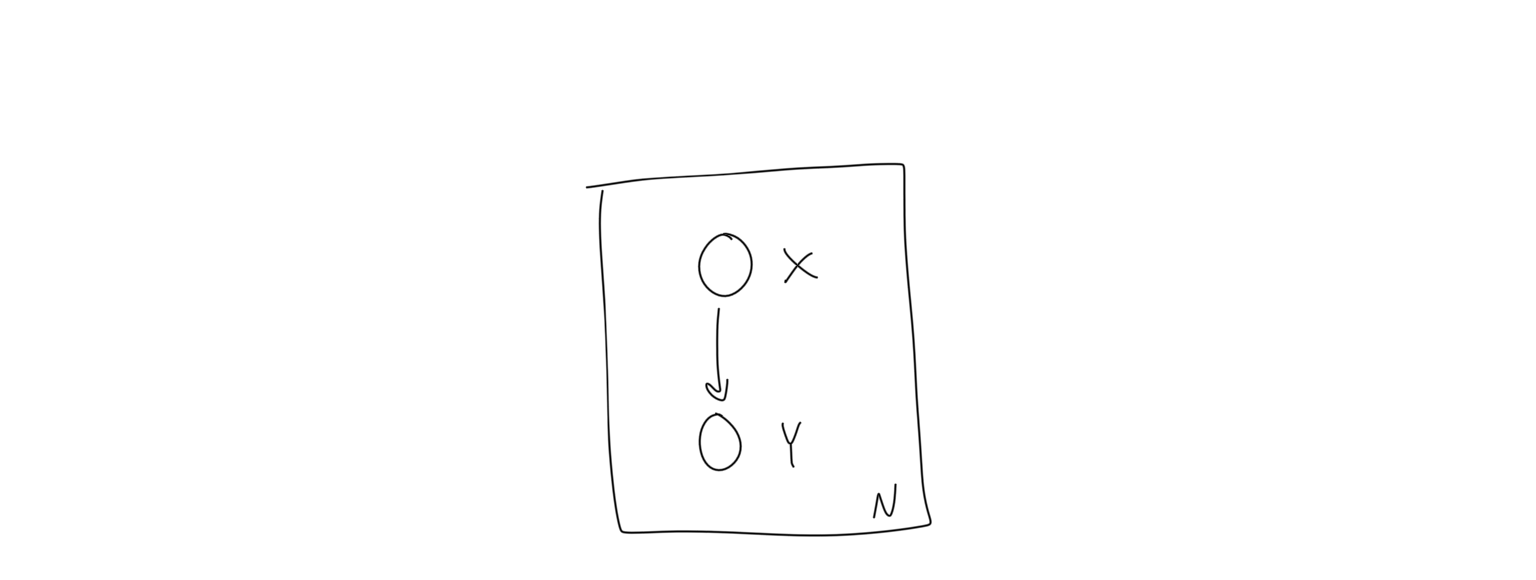
\includegraphics[width=0.7\paperwidth]{../GraphicalModels/fig/plates.png}
    \caption{Plates indicate repeated sets of variables. Often there will be a number in one of the corners (N in this case) indicating how many times that variable is repeated.}
    \label{fig:plates}
\end{figure}

First, we have random variables represented by an open circle, shown in Figure \ref{fig:random-var}. Note that if we observe a random variable of a given model, then we shade it in. Otherwise, it's left open.

Second, we have deterministic parameters represented by a tight, small dot, shown in Figure \ref{fig:deterministic-param}.

Third, we have arrows that indicate the dependence relationship between different random variables and parameters, shown in Figure \ref{fig:arrows}. Note that an arrow from $X$ into $Y$ means that $Y$ depends on $X$.

And finally, we have plate notation to indicate that we have repeated sets of variables in our model setup, shown in Figure \ref{fig:plates}.

With these four simple constructs, we can describe complex model setups with a simple diagram. We can have an arbitrary number of component with any sort of dependence structure baked in. DGMs can be useful as a reference while working on a problem, and they also make it easy to iterate on an existing model setup.

\subsection{Joint Probability Distributions}
We'll now consider how DGMs simplify the task of reasoning about a joint probability distribution over multiple random variables. Note that for any joint probability distribution, regardless of our knowledge about the dependence structure in the model, it's always valid to write a generic joint probability distribution as follows:
\begin{align*}
	p(A, B, C)
\end{align*}
where in this setup, we are interested in the joint distribution between three random variables $A, B, C$. However, this doesn't tell us anything about the structure of the problem at hand: where there is independence and how we can use that to simplify our model. For example, if we knew that $B$ and $C$ were independent and we also knew the conditional distribution of $A | B, C$ then we would much rather setup our joint probability equation as:
\begin{equation} \label{joint-distr-example}
	p(A, B, C) = p(B)p(C)p(A | B, C)
\end{equation}
DGMs assist in this process of identifying the appropriate factorization, as their structure allows us to read off valid factorizations directly. For example, the joint distribution given by Equation \ref{joint-distr-example} can be read from Figure \ref{fig:joint-distr-example-dgm}.
\begin{figure}
    \centering
    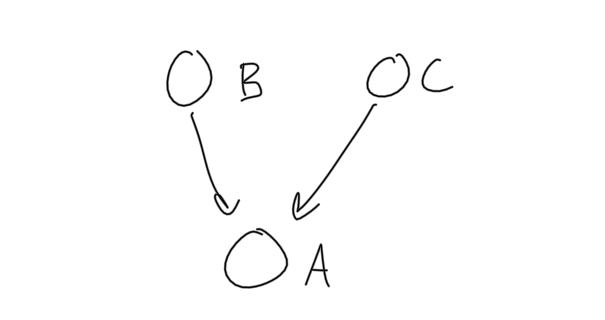
\includegraphics[width=0.5\paperwidth]{../GraphicalModels/fig/joint-distr-example-dgm.png}
    \caption{DGM for the joint distribution give by Equation \ref{joint-distr-example}.}
    \label{fig:joint-distr-example-dgm}
\end{figure}

We can move between a DGM and a valid factorized joint distribution by identifying the arrows indicating dependencies. If a random variable has no dependencies (as neither $B$ nor $C$ do in this example), they can be written on their own as marginal probabiilties $p(B)$ and $p(C)$. For random variables with arrows coming into them, indicating dependence, we include them in the joint factorization conditioned on the variables that they depend on, i.e. $P(A | B, C)$. In this way we can move back and forth between DGMs and factorized joint distributions with ease.

\subsection{Generative Models}
While DGMs allow us to move quickly between a factorized joint distribution and a corresponding graphical model, they also show us the process by which data comes into existence (sometimes referred to as the data generating story or generative process). What this means is that if presented with a DGM, it is possible for us to identify how the data gets created, and if we have the proper tools, how we could generate new data ourselves.

\begin{definition}{Generative Models}{generative-models}
    A generative model describes the entire process by which data comes into existence. While this is not always necessary if our goal is only to make predictions or perform some other kind of inference, it does have the added benefit of enabling the creation of new data by sampling from the generative model.
\end{definition}

\readernote{Note that we can create graphical models for both generative and discriminative models. Discriminative models will only model the conditional distribution $p(Y|Z)$, while generative models will model the full joint distribution $p(Z, Y)$.}

Let's consider a simple example to see how this works in practice.
\begin{figure}
    \centering
    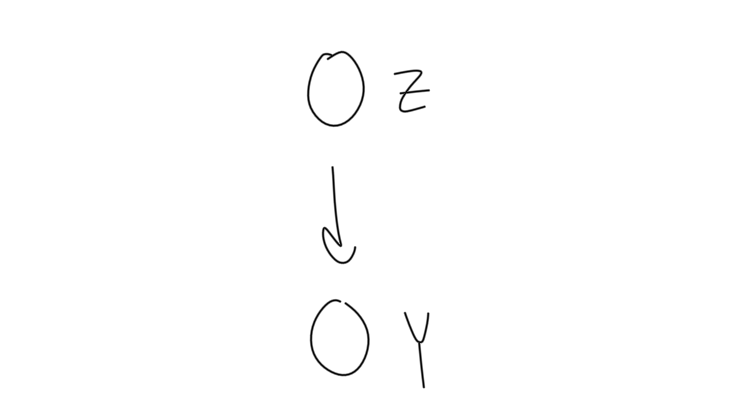
\includegraphics[width=0.5\paperwidth]{../GraphicalModels/fig/GenerativeRVExample.png}
    \caption{Example of a generative model.}
    \label{fig:generative-rv}
\end{figure}
Consider the flow of information present in Figure \ref{fig:generative-rv}. First, there is some realization of the random variable $Z$. Then conditioned on that value of $Z$, there is some realization of the random variable $Y$. Obviously, the joint factorization for this DGM is given by $p(Z)p(Y|Z)$, but on a more intuitive level, the data is created by first sampling from $Z$'s distribution, and then based on that value, sampling from the conditional distribution of $Y$.

To make this concrete, we could consider $Z$ to be a random variable that determines a specific breed of dog, and $Y$ to be the random variable that, conditioned on the breed of dog, determines the snout length of that type of dog. Notice that we have not specified anything about the specific distributional form from which $Z$ and $Y$ come, only the story of how they relate to each other.

This story also shows us that if we had some model for $Z$ and $Y|Z$, we could generate data points ourselves. Our procedure would simply be to sample from $Z$ and then to sample from $Y$ conditioned on that value of $Z$. We could perform this process as many times as we like to generate new data. This is in contrast to sampling directly from the joint $p(Z, Y)$, which is difficult if we don't know the exact form of the joint distribution (which we often do not) or if the joint distribution is hard to sample from directly.

The technique of sampling from distributions in the order indicated by their DGM is known as \textbf{ancestral sampling}, and it is a major benefit of generative models.

\begin{definition}{Ancestral Sampling}{ancestral-sampling}
	Ancestral sampling is a technique used to generate data from an arbitrary DGM. It works by sampling from the random variables in topological order, meaning that we first sample from all random variables without any dependence, then from the random variables that depend on those intially sampled random variables, and so on until all the random variables have been sampled. This is demonstrated in Figure \ref{fig:ancestral-sampling}.
\end{definition}
\begin{figure}
	\centering
	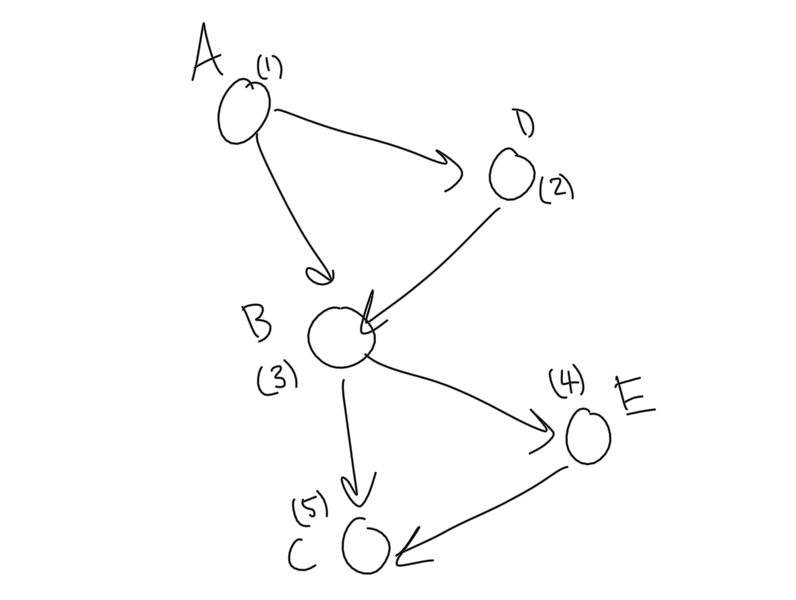
\includegraphics[width=0.5\paperwidth]{../GraphicalModels/fig/AncestralSampling.png}
    \caption{Notice we have to sample these in topological order: A, D, B, E, C.}
	\label{fig:ancestral-sampling}
\end{figure}

\subsection{Generative Modeling vs. Discriminative Modeling}
In the previous section, we described generative modeling. You may have wondered if there was any other type of modeling possible, if not the model that describes how data comes into existence. There is another type of model known as a discriminative model, and we have already seen several examples of them.

A discriminitive model skips the step of describing how data was generated (i.e. it doesn't model the joint $p(Z, Y)$), and instead it cuts right to our predictive objective (i.e. it models the conditional $p(Y|Z)$). For example, if we wish to predict what value a response variable will take on, we can consider the input data points to be parameters without an underlying distribution, and then our model is simply tasked with predicting the response variable based on those parameters. This is in contrast to a generative model, which would model how all the various data points came into existence by assigning a distribution to each of them.

Discriminative modeling is exactly what we did with linear and logistic regression, and it's commonly what we do with SVMs and neural networks as well. Let's consider the DGM describing linear regression again, from Figure \ref{fig:lin-reg-dgm}. Notice that the data points $\textbf{x}_n$ are not random variables but merely parameters of the DGM. If we wanted a generative model, we would instead have a DGM that looks that of Figure \ref{fig:lin-reg-model-x}.
\begin{figure}
	\centering
	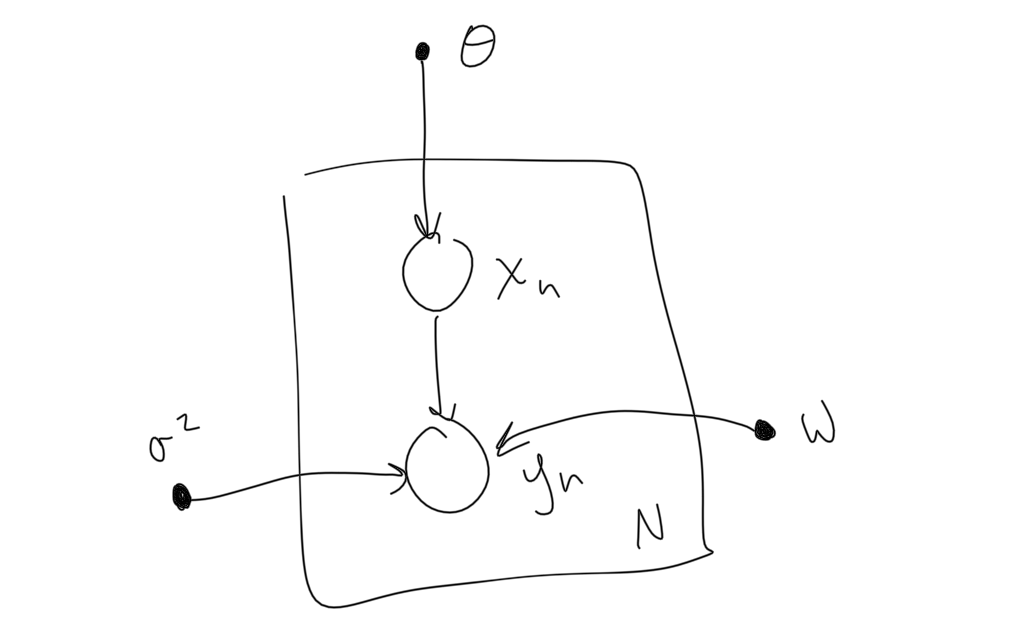
\includegraphics[width=0.5\paperwidth]{../GraphicalModels/fig/lin-reg-model-x.png}
    \caption{Linear regression DGM, modeling $\textbf{x}_n$ as a random variable.}
	\label{fig:lin-reg-model-x}
\end{figure}

The difference between these model setups is significant. The generative model for linear regression would allow us to generate new data points, but it is also significantly more complex to handle because now instead of having just a single response variable to predict, we also have to contend with how we model the generation of the data points $\textbf{x}_n$. This may be difficult on both conceptual and computational levels. This doesn't mean we'll never try to do this, but if our goal is simply to make predictions about the response variable $y_n$, it may be overkill to use a generative model.

In essence, the distinction between generative and discriminative models comes down to whether or not the model tries to describe how the data is realized or if the model simply tries to perform a specific inference task without modeling the entirety of the data generating process. Neither one is better, they are just different techniques that will apply differently depending on your modeling and inferential needs.

\subsection{Understanding Complexity}
We've already motivated one of the primary uses of DGMs as being the ability to convert a joint distribution into a factorization. At the heart of that task was recognizing and exploiting independence properties in a model over multiple random variables. Another benefit of this process is that it allows us to easily reason about the size (also called `complexity') of a joint factorization over discrete random variables. In other words, it allows us to determine how many parameters we will have to learn to describe the factorization for a given DGM.

Let's consider an example to make this concept clear. Let's say we have four categorical random variables A, B, C, D which take on 2, 4, 8, and 16 values respectively. If we were to assume full dependence between each of these random variables, then a joint distribution table over all of these random variables would require $(2 * 4 * 8 * 16) - 1$ total parameters (where each parameter corresponds to the probability of a specific permutation of the values A, B, C, D).

\readernote{Notice that the number of parameters we need is $(2 * 4 * 8 * 16) - 1$ and not $(2 * 4 * 8 * 16)$. This is simply because if we know the first $(2 * 4 * 8 * 16) - 1$ parameters, we can calculate the value of the final one exactly.}

However, if we knew that some of these random variables were conditionally independent, then the number of parameters would change. For example, consider the joint distribution given by $p(A, B, C, D) = p(A)p(B|A)p(C|A)p(D|A)$. This would imply that conditioned on $A$, each of $B, C, D$ were conditionally independent. This can also be shown by the DGM in Figure \ref{fig:complexity-dgm}.
\begin{figure}
	\centering
	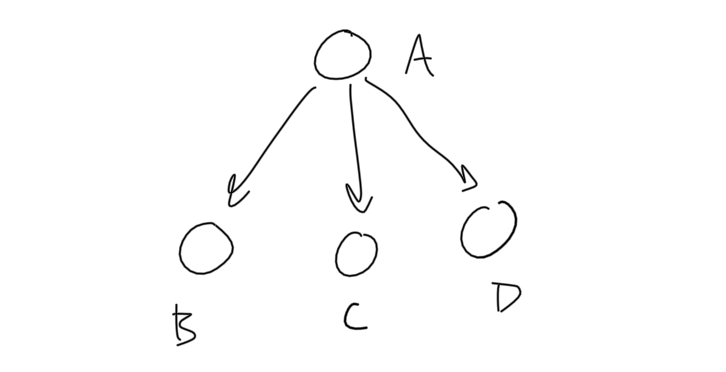
\includegraphics[width=0.5\paperwidth]{../GraphicalModels/fig/complexity-dgm.png}
    \caption{Conditioned on A, we have that B, C, and D are independent.}
	\label{fig:complexity-dgm}
\end{figure}

In this case, a table of parameters to describe this joint distribution would only require $2 * ((4 - 1) + (8 - 1) + (16 - 1))$ parameters, which is significantly less.

This leads to the natural conclusion that the more conditional independence we can identify in a given model, the easier it becomes from a modeling and computational perspective. This is another major benefit of DGMs: it's possible to visually reason about the independence properties of a given model. We turn to how this works next.

\subsection{Independence and D-Separation}
We can use the form of a graphical model directly to determine which variables are independent under specific observation assumptions. We have three base cases for the relationship between variables from which we can reason about the structure in any arbitrarily complex model. The three cases look like what's found in Figure \ref{fig:indep-structure}.
\begin{figure}
	\centering
	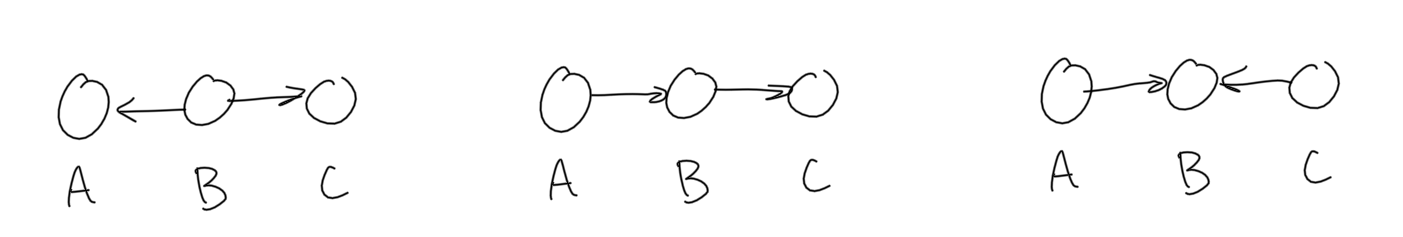
\includegraphics[width=0.5\paperwidth]{../GraphicalModels/fig/indep-structure.png}
    \caption{The three random variable relationships that will tell us about independence relationships.}
	\label{fig:indep-structure}
\end{figure}
For each of these cases, there is a notion of information either flowing from one random variable to the other or being `blocked' (implying independence) by an observation. Specifically, case 1 and case 2 have information between nodes A and C `blocked' by observing node B, and case 3 has information between nodes A and C `blocked' by \textit{not} observing node B.

Let's consider each of these cases more carefully, and gain a better notion of what it means for observations to cause information to be blocked. This will lead naturally to an understanding of independence assumptions between random variables. Considering the first example random variable structure, shown in Figure \ref{fig:first-case-unobserved}.

\begin{figure}
	\centering
	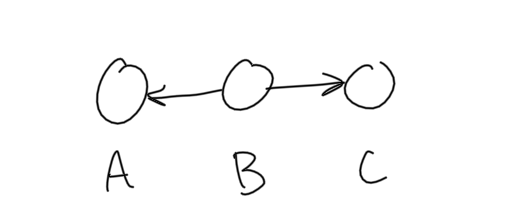
\includegraphics[width=0.5\paperwidth]{../GraphicalModels/fig/first-case-unobserved.png}
	\caption{First structure, unobserved.}
	\label{fig:first-case-unobserved}
\end{figure}

We can factorize this as follows:
\begin{align*}
	p(A, B, C) = p(B) p(A | B) p(C | B)
\end{align*}

We know that for this case, A and C are not independent (note that we have not observed B). Therefore, we say that information flows from A to C. However, once we've observed B, we have that A and B are conditionally independent, shown in Figure \ref{fig:first-case-observed}.

\begin{figure}
	\centering
	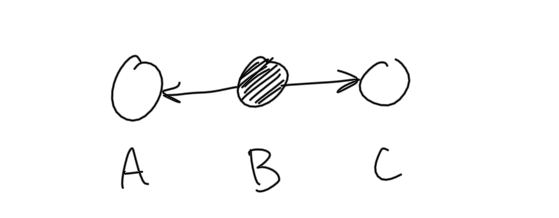
\includegraphics[width=0.5\paperwidth]{../GraphicalModels/fig/first-case-observed.png}
	\caption{First structure, observed.}
	\label{fig:first-case-observed}
\end{figure}

We now say that the flow of information from A to C is `blocked' by the observation of B. Thus they are conditionally independent. Intuitively, if we observe A but not B, then we have some information about what B might be and therefore also what C might be. The same applies in the other direction: observing C but not B.

Moving on to the second random variable structure, shown in Figure \ref{fig:second-case-unobserved}, we again consider the unobserved case first.
\begin{figure}
	\centering
	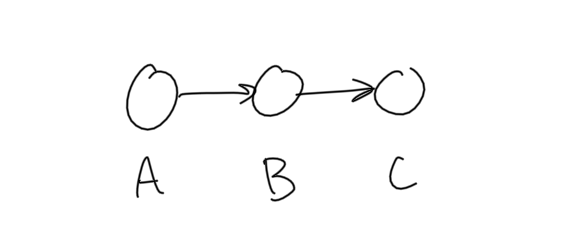
\includegraphics[width=0.5\paperwidth]{../GraphicalModels/fig/second-case-unobserved.png}
	\caption{Second structure, unobserved.}
	\label{fig:second-case-unobserved}
\end{figure}

This allows us to write the joint distribution as:

\begin{align*}
	p(A, B, C) = p(A) p(B | A) p(C | B)
\end{align*}

We have that for this case, A and C are not independent if we have not observed C. Information is flowing from A to B through C. However, once we've observed B, then we have that A and C are again conditionally independent, shown in Figure \ref{fig:second-case-observed}.

\begin{figure}
	\centering
	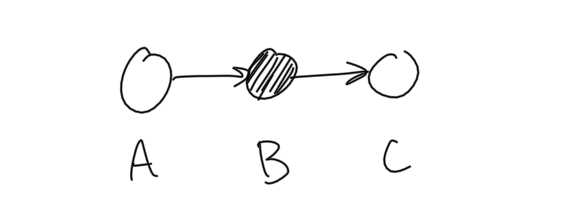
\includegraphics[width=0.5\paperwidth]{../GraphicalModels/fig/second-case-observed.png}
	\caption{Second structure, observed.}
	\label{fig:second-case-observed}
\end{figure}

We again say that the flow of information from A to C is `blocked' by the observation of B. Intuitively, if we observed A but not B, we have some information about what B might be and therefore what C might be as well.  The same applies in the other direction: observing C but not B.

Notice that these first two cases behave in the same manner: observing a random variable in between two other random variable `blocks' information from flowing between the two outer random variables. In the third and final case the opposite is true. Not observing data in this case will `block' information, and we will explain this shift through an idea known as `explaining away'.

We have the third and final random variable structure, shown in Figure \ref{fig:third-case-unobserved}. We consider the unobserved case first.
\begin{figure}
	\centering
	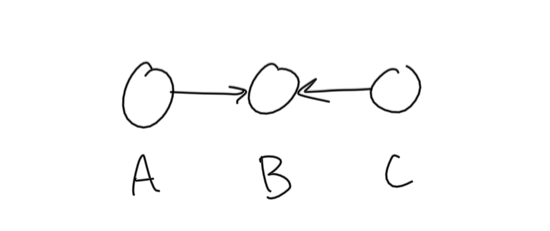
\includegraphics[width=0.5\paperwidth]{../GraphicalModels/fig/third-case-unobserved.png}
	\caption{Third structure, unobserved.}
	\label{fig:third-case-unobserved}
\end{figure}

In this setup, we say that information from A to C is being `blocked' by the unobserved variable B. Thus A and C are currently conditionally independent. However, once we've observed B, as shown in Figure \ref{fig:third-case-observed}, the information flow changes.
\begin{figure}
	\centering
	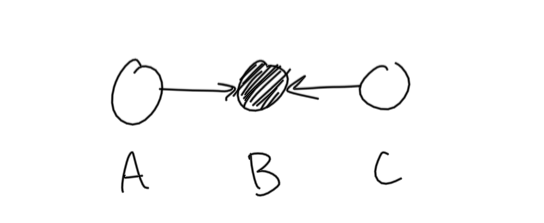
\includegraphics[width=0.5\paperwidth]{../GraphicalModels/fig/third-case-observed.png}
	\caption{Third structure, observed.}
	\label{fig:third-case-observed}
\end{figure}

Now, information is flowing between A and C through the observed variable B, and thus A and C are now conditionally dependent. This phenomenon, where the observation of the random variable in the middle creates conditional dependence is known as \textit{explaining away}. The idea relies on the fact that now that we know the value for B, we have some idea of how much A or C may have contributed to B adopting that value. An example might make this phenomenon more clear.

Let's consider that the random variable A corresponds to whether or not it rained on a certain day, the random variable B corresponds to the lawn being wet, and the random variable C corresponds to the sprinkler being on. Let's say we observe B: the lawn is wet. Let's say we then observe variable A: it has not rained today. Intuitively, we would now assume that variable C would have the value that the sprinkler has been on, because that's the only way for the lawn to be wet. This is exactly the phenomenon of explaining away. Observing B unblocks the flow of information between A and C because we can now use an observation to `explain' how B got its value, and therefore determine what the other unobserved value might have been.

Notice that we've only described three simple cases relating dependence relationships between random variables in a DGM, but with just these three cases, we can determine the dependence structure of any arbitrarily complicated DGM. We just have to consider how information flows from node to node. If information gets `blocked' at any point in our DGM network because of an observation (or lack thereof), then we gain some knowledge about independence within our model.

Consider the dependence between random variables A and F in Figure \ref{fig:information-flow-example}. Initially, before any observations are made, we can see that A and F are dependent (information flows from A through B). However, after observing B, A and F become independent (because information blocked at both the observed B and unobserved D). Finally, after observing D, A and F are once again dependent. Now we have information that flows from A through D.
\begin{figure}
	\centering
	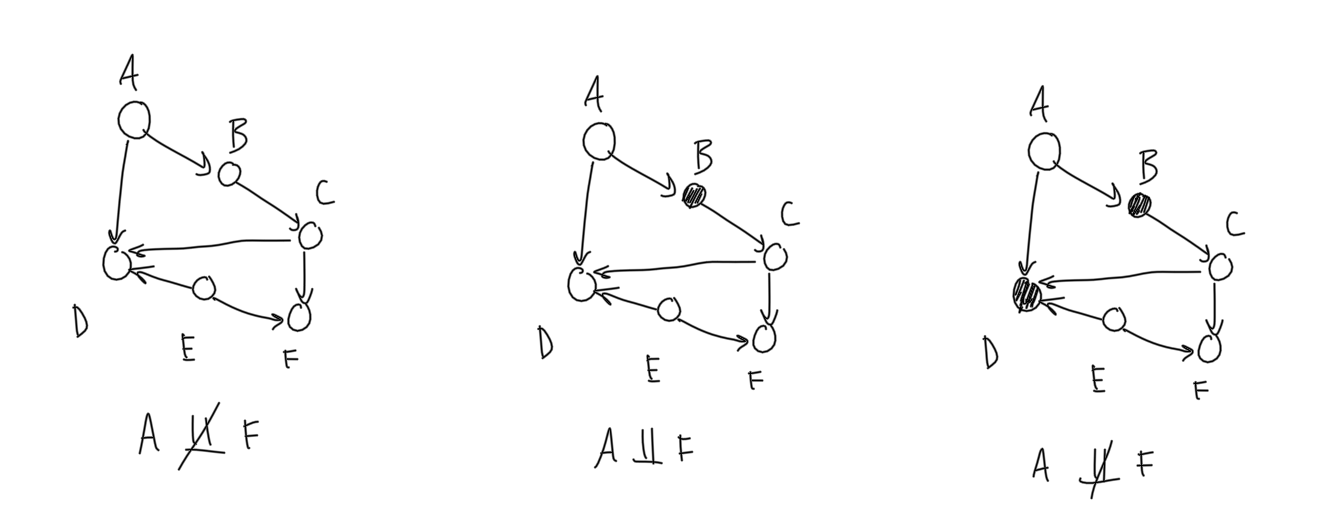
\includegraphics[width=0.5\paperwidth]{../GraphicalModels/fig/information-flow-example.png}
    \caption{Notice how the independence between A and F depends on observations made within the network.}
	\label{fig:information-flow-example}
\end{figure}

\readernote{In some other resources, you'll come upon the idea of `D-separation' or `D-connection'. D-separation is simply applying the principles outlined above to determine if two nodes are independent, or D-separated. On the other hand, two-nodes that are D-connected are dependent on one another.}

\section{Example: Naive Bayes}
Recall from the chapter on classification the Naive Bayes model. As a quick recap, Naive Bayes makes the assumption that for a single observation coming from a specific class (for example, our classes could be different dog breeds), the data associated with that observation are independent (for example, the data could be fur color, snout length, weight, etc.).

We can set up the Naive Bayes problem specification using the DGM form, as we see in Figure \ref{fig:naive-bayes}.
\begin{figure}
	\centering
	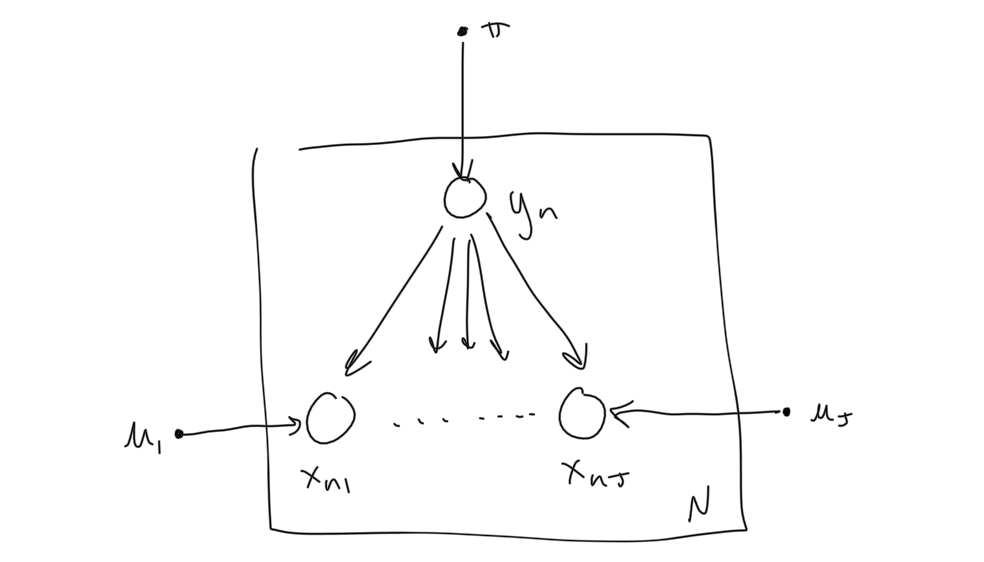
\includegraphics[width=0.5\paperwidth]{../GraphicalModels/fig/naive-bayes-dgm.png}
    \caption{DGM for Naive Bayes problem setup.}
	\label{fig:naive-bayes}
\end{figure}

Even if we hadn't heard of Naive Bayes before, we would understand this model and the implications of the model, simply by an examination of the DGM that describes it. We can directly read off the factorization described above that is the whole point of Naive Bayes:
\begin{align*}
	p(y_n, x_{n1}, ..., x_{nJ}) = p(y_n) p(x_{n1} | y_n) \cdot \cdot \cdot p(x_{nJ} | y_n)
\end{align*}
Writing this factorization is facilitated directly by our DGM, even if we've never heard of Naive Bayes before. It provides a common language for us to move fluidly between detailed probability factorizations and general modeling intuition.

\section{Conclusion}
Directed graphical models are indispensible for model visualization and effective communication of modeling ideas. With an understanding of what DGMs are meant to represent, it's much easier to dig into more complex probabilistic models. In a lot of ways, this chapter is preparation for where we head next. The topics of the following chapters will rely heavily on DGMs to explain their structure, use cases, and interesting variants.